%!TeX root=../tese.tex
%("dica" para o editor de texto: este arquivo é parte de um documento maior)
% para saber mais: https://tex.stackexchange.com/q/78101/183146

%% ------------------------------------------------------------------------- %%
\chapter{Retângulos independentes}
\label{cap:retângulos-independentes}

\newcommand{\rectpos}{%
    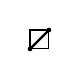
\begin{tikzpicture}[baseline={(0,0)}, scale=0.2]
        \draw (0,0) rectangle (1.2,1.2); % Quadrado
        \draw[thick] (0,0) -- (1.2,1.2); % Diagonal
        \fill (0,0) circle (0.15); % Ponto no início da diagonal
        \fill (1.2,1.2) circle (0.15); % Ponto no fim da diagonal
    \end{tikzpicture}%
}

\newcommand{\rectneg}{%
    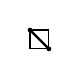
\begin{tikzpicture}[baseline={(0,0)}, scale=0.2]
        \draw (0,0) rectangle (1.2,1.2); % Quadrado
        \draw[thick] (0,1.2) -- (1.2,0); % Diagonal (invertida)
        \fill (0,1.2) circle (0.15); % Ponto no início da diagonal
        \fill (1.2,0) circle (0.15); % Ponto no fim da diagonal
    \end{tikzpicture}%
}

\newcommand{\recttotal}{%
    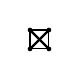
\begin{tikzpicture}[baseline={(0,0)}, scale=0.2]
        \draw (0,0) rectangle (1.2,1.2); % Quadrado
        \draw[thick] (0,1.2) -- (1.2,0); % Diagonal (invertida)
        \draw[thick] (0,0) -- (1.2,1.2); % Diagonal
        \fill (0,1.2) circle (0.15); % Ponto no início da diagonal
        \fill (1.2,0) circle (0.15); % Ponto no fim da diagonal
        \fill (0,0) circle (0.15); % Ponto no início da diagonal
        \fill (1.2,1.2) circle (0.15); % Ponto no fim da diagonal
    \end{tikzpicture}%
}

Neste capítulo entenderemos como utilizar a visão geométrica da execução de um algoritmo de busca em ABB para delimitar inferiormente custos em sequências de acesso. Introduziremos as noções de orientação e independência de retângulos que serão fundamentais para a elaboração e análise dos algoritmos gulosos futuristas orientados. Explicaremos como funciona a delimitação dos retângulos independentes e por fim faremos um estudo da qualidade dessa delimitação inferior.

\section{Orientação de retângulos}
%\section{Categoria de retângulos}

Para construção de provas mais sofisticadas, é necessário entender melhor características da geometria dos retângulos formados por pontos de um conjunto. Lembre-se que todos os retângulos aqui considerados são ortogonais aos eixos cartesianos. Por conveniência das provas, todas as sequências de acessos desse capítulo possuem tamanho $n$ e todas as chaves são buscadas exatamente uma vez, ou seja, a sequência de busca é uma permutação de 1 a $n$.

Dividiremos os retângulos formados por um par de pontos de um conjunto $P$ em dois grupos, os $\rectpos$-retângulos e os $\rectneg$-retângulos. Denotamos por $\rectpos$\textit{-retângulo} os retângulos que possuem o vértice à esquerda mais abaixo que o vértice à direita. Denotamos por $\rectneg$\textit{-retângulo} os retângulos que possuem o vértice à esquerda mais acima que o vértice à direita.

Assim, definimos que um conjunto de pontos $P$ é $\rectpos$\textit{-satisfeito} se todos os $\rectpos$-retângulos formados por dois pontos de $P$ não ortogonalmente colineares são arboreamente satisfeitos. O conceito de $\rectneg$-satisfeito é definido simetricamente.

Também será útil definir quando ambos os tipos de retângulos são satisfeitos. Chamamos um superconjunto $Z$ de $P$ de $\recttotal$\textit{-satisfeito} em relação a $P$ se existem subconjuntos $Z_{\rectpos}$ e $Z_{\rectneg}$ de $Z$ tais que $Z_{\rectpos} \cup P$ é $\rectpos$-satisfeito e $Z_{\rectneg} \cup P$ é $\rectneg$-satisfeito.  

%todos os $\rectpos$-retângulos e os $\rectneg$-retângulos são arboreamente satisfeitos, ou seja, $X$ é $\rectpos$-satisfeito e $\rectneg$-satisfeito.

Por fim, definimos \textit{minASS}$_{\rectpos}(P)$ como o tamanho de um menor superconjunto de $P$ que é $\rectpos$-satisfeito. Analogamente, \textit{minASS}$_{\rectneg}(P)$ é o tamanho de um menor superconjunto de $P$ que é $\rectneg$-satisfeito e \textit{minASS}$_{\recttotal}(P)$ é o tamanho do menor superconjunto de $P$ que é $\recttotal$-satisfeito em relação a $P$.

%EXPLICAR MAIS!! NAO ESTÁ CLARA A CONCLUSÃO DA EQUAÇÃO.
Note que qualquer união entre dois conjuntos $Z_{\rectpos}$ e $Z_{\rectneg}$, onde $Z_{\rectpos}$ é $\rectpos$-satisfeito, $Z_{\rectneg}$ é $\rectneg$-satisfeito e ambos são superconjuntos de $P$, é $\recttotal$-satisfeita em relação a $P$. Veja Figura~\ref{fig:eq4.1_ex_minimal}. Porém, $Z_{\rectpos} \setminus P$ e $Z_{\rectneg} \setminus P$ não necessariamente são disjuntos entre si. Levando em consideração ambas as propriedade, conclui-se então a Equação~\ref{eq:minASStotal_menorouigual_soma_de_minASSs}.
\begin{equation} \label{eq:minASStotal_menorouigual_soma_de_minASSs}
    \text{minASS}_{\recttotal}(P) \leq \text{minASS}_{\rectpos}(P) + \text{minASS}_{\rectneg}(P).
\end{equation}

\begin{figure}
    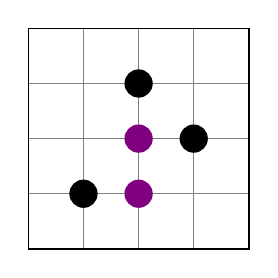
\begin{tikzpicture}[scale=0.7]
        \draw[very thin, gray] (0,0) grid (4,4);

        \filldraw[black] (1,1) circle (7pt);
        \filldraw[black] (2,3) circle (7pt);
        \filldraw[black] (3,2) circle (7pt);
        \filldraw[violet] (2,1) circle (7pt);
        \filldraw[violet] (2,2) circle (7pt);
        
        \draw[black, line width=0.5pt] (0,0) rectangle (4,4);
    \end{tikzpicture}
    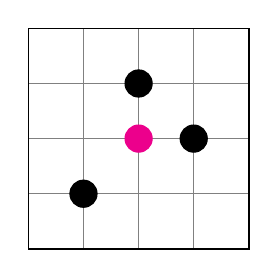
\begin{tikzpicture}[scale=0.7]
        \draw[very thin, gray] (0,0) grid (4,4);

        \filldraw[black] (1,1) circle (7pt);
        \filldraw[black] (2,3) circle (7pt);
        \filldraw[black] (3,2) circle (7pt);
        \filldraw[magenta] (2,2) circle (7pt);
        
        \draw[black, line width=0.5pt] (0,0) rectangle (4,4);
    \end{tikzpicture}
    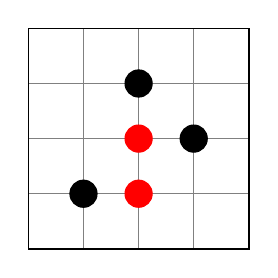
\begin{tikzpicture}[scale=0.7]
        \draw[very thin, gray] (0,0) grid (4,4);

        \filldraw[black] (1,1) circle (7pt);
        \filldraw[black] (2,3) circle (7pt);
        \filldraw[black] (3,2) circle (7pt);
        \filldraw[red] (2,1) circle (7pt);
        \filldraw[red] (2,2) circle (7pt);
        
        \draw[black, line width=0.5pt] (0,0) rectangle (4,4);
    \end{tikzpicture}
    \caption{Em preto, os pontos de $P_X$ para a sequência de acessos $X = (1,3,2)$. À esquerda, em roxo, um conjunto de pontos $Z_{\protect\rectpos}$, onde $Z_{\protect\rectpos} \cup P_X$ é $\protect\rectpos$-satisfeito e possui tamanho minASS$_{\protect\rectpos}$. Ao centro, em rosa, um conjunto de pontos $Z_{\protect\rectneg}$, onde $Z_{\protect\rectneg} \cup P_X$ é $\protect\rectneg$-satisfeito e possui tamanho minASS$_{\protect\rectneg}$. À direita, em vermelho, um conjunto de pontos $Z_{\protect\recttotal}$, onde $Z_{\protect\recttotal} \cup P_X$ é $\protect\rectpos$-satisfeito e $\protect\rectneg$-satisfeito e possui tamanho minASS$_{\protect\recttotal}$. Perceba que $Z_{\protect\recttotal} = Z_{\protect\rectpos} \cup Z_{\protect\rectneg}$ e $Z_{\protect\rectpos} \cap Z_{\protect\rectneg} \neq \emptyset$.}
\label{fig:eq4.1_ex_minimal}
\end{figure}

Outro ponto fundamental de ser compreendido é que todo conjunto $Y$, superconjunto de $P$, arboreamente satisfeito também é $\recttotal$-satisfeito em relação a $P$. Isso acontece pois por conta do conjunto $Y$ ser superconjunto de $P$ e arboreamente satisfeito, então $Y \cup P = Y$ que é $\rectpos$-satisfeito e $\rectneg$-satisfeito. Assim, temos que
\begin{equation} \label{eq:minASS_orientado_menor_ou_igual_minASS}
    \text{minASS}_{\recttotal}(P) \leq \text{minASS}(P).
\end{equation}

\section{Guloso futurista orientado}

Definimos agora dois algoritmos muito parecidos com o guloso futurista visto no capítulo anterior, que nos ajudarão a descrever delimitações inferiores em buscas. 

Chamaremos de guloso \textit{futurista}-$\rectpos$ o seguinte algoritmo que recebe um conjunto $P_X$ de pontos que representa uma sequência $X$ de buscas. O algoritmo começa com $P = P_X$ e desliza uma reta horizontal $r$ que começa em $y = 1$ e vai até $y = m$. O algoritmo mantém o invariante que todos os pares de pontos de $P$ em $r$ ou abaixo de $r$ são $\rectpos$-satisfeitos. Esse algoritmo garante essa propriedade adicionando a $P$ o menor número de pontos na linha $r$ durante cada iteração. Ao fim da execução, o conjunto $P$ de pontos é $\rectpos$-satisfeito. O algoritmo guloso futurista-$\rectneg$ é definido de maneira simétrica considerando a $\rectneg$-satisfação.

Chamaremos de Fut$_{\rectpos}(P)$ o conjunto de pontos adicionados durante a execução do algoritmo guloso futurista-$\rectpos$ para um conjunto $P$ de pontos. Todas essas definições valem simetricamente para o algoritmo guloso futurista-$\rectneg$.
Veja a Figura~\ref{fig:greedy_sign}.

\begin{figure}
    \centering
    \begin{minipage}[b]{0.48\linewidth}
        \centering
        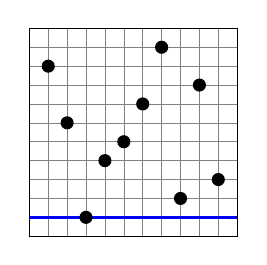
\begin{tikzpicture}[scale=0.24]
            \draw[very thin, gray] (0,0) grid (11,11);
    
            \draw[blue, line width=1.2pt] (0,1) -- (11,1);

            \filldraw[black] (3,1) circle (9pt);
            \filldraw[black] (8,2) circle (9pt);
            \filldraw[black] (10,3) circle (9pt);
            \filldraw[black] (4,4) circle (9pt);
            \filldraw[black] (5,5) circle (9pt);
            \filldraw[black] (2,6) circle (9pt);
            \filldraw[black] (6,7) circle (9pt);
            \filldraw[black] (9,8) circle (9pt);
            \filldraw[black] (1,9) circle (9pt);
            \filldraw[black] (7,10) circle (9pt);
            \draw[black, line width=0.5pt] (0,0) rectangle (11,11); 
        \end{tikzpicture}
        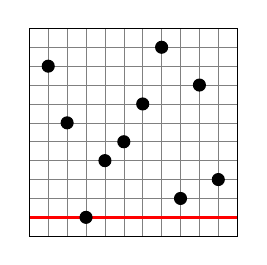
\begin{tikzpicture}[scale=0.24]
            \draw[very thin, gray] (0,0) grid (11,11);
    
            \draw[red, line width=1.2pt] (0,1) -- (11,1);

            \filldraw[black] (3,1) circle (9pt);
            \filldraw[black] (8,2) circle (9pt);
            \filldraw[black] (10,3) circle (9pt);
            \filldraw[black] (4,4) circle (9pt);
            \filldraw[black] (5,5) circle (9pt);
            \filldraw[black] (2,6) circle (9pt);
            \filldraw[black] (6,7) circle (9pt);
            \filldraw[black] (9,8) circle (9pt);
            \filldraw[black] (1,9) circle (9pt);
            \filldraw[black] (7,10) circle (9pt);

            \draw[black, line width=0.5pt] (0,0) rectangle (11,11); 
        \end{tikzpicture}
        \\
        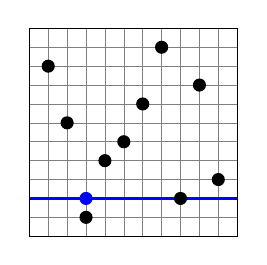
\begin{tikzpicture}[scale=0.24]
            \draw[very thin, gray] (0,0) grid (11,11);
    
            \draw[blue, line width=1.2pt] (0,2) -- (11,2);

            \filldraw[black] (3,1) circle (9pt);
            \filldraw[black] (8,2) circle (9pt);
            \filldraw[black] (10,3) circle (9pt);
            \filldraw[black] (4,4) circle (9pt);
            \filldraw[black] (5,5) circle (9pt);
            \filldraw[black] (2,6) circle (9pt);
            \filldraw[black] (6,7) circle (9pt);
            \filldraw[black] (9,8) circle (9pt);
            \filldraw[black] (1,9) circle (9pt);
            \filldraw[black] (7,10) circle (9pt);

            \filldraw[blue] (3,2) circle (9pt);

            \draw[black, line width=0.5pt] (0,0) rectangle (11,11); 
        \end{tikzpicture}
        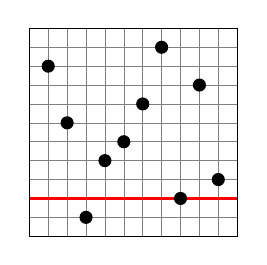
\begin{tikzpicture}[scale=0.24]
            \draw[very thin, gray] (0,0) grid (11,11);
    
            \draw[red, line width=1.2pt] (0,2) -- (11,2);

            \filldraw[black] (3,1) circle (9pt);
            \filldraw[black] (8,2) circle (9pt);
            \filldraw[black] (10,3) circle (9pt);
            \filldraw[black] (4,4) circle (9pt);
            \filldraw[black] (5,5) circle (9pt);
            \filldraw[black] (2,6) circle (9pt);
            \filldraw[black] (6,7) circle (9pt);
            \filldraw[black] (9,8) circle (9pt);
            \filldraw[black] (1,9) circle (9pt);
            \filldraw[black] (7,10) circle (9pt);

            \draw[black, line width=0.5pt] (0,0) rectangle (11,11); 
        \end{tikzpicture}
        \\
        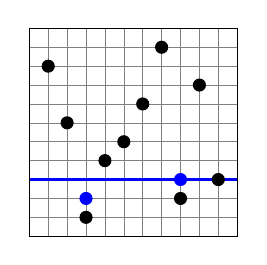
\begin{tikzpicture}[scale=0.24]
            \draw[very thin, gray] (0,0) grid (11,11);
    
            \draw[blue, line width=1.2pt] (0,3) -- (11,3);

            \filldraw[black] (3,1) circle (9pt);
            \filldraw[black] (8,2) circle (9pt);
            \filldraw[black] (10,3) circle (9pt);
            \filldraw[black] (4,4) circle (9pt);
            \filldraw[black] (5,5) circle (9pt);
            \filldraw[black] (2,6) circle (9pt);
            \filldraw[black] (6,7) circle (9pt);
            \filldraw[black] (9,8) circle (9pt);
            \filldraw[black] (1,9) circle (9pt);
            \filldraw[black] (7,10) circle (9pt);

            \filldraw[blue] (3,2) circle (9pt);
            \filldraw[blue] (8,3) circle (9pt);

            \draw[black, line width=0.5pt] (0,0) rectangle (11,11); 
        \end{tikzpicture}
        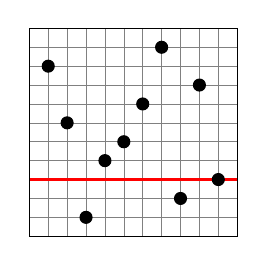
\begin{tikzpicture}[scale=0.24]
            \draw[very thin, gray] (0,0) grid (11,11);
    
            \draw[red, line width=1.2pt] (0,3) -- (11,3);

            \filldraw[black] (3,1) circle (9pt);
            \filldraw[black] (8,2) circle (9pt);
            \filldraw[black] (10,3) circle (9pt);
            \filldraw[black] (4,4) circle (9pt);
            \filldraw[black] (5,5) circle (9pt);
            \filldraw[black] (2,6) circle (9pt);
            \filldraw[black] (6,7) circle (9pt);
            \filldraw[black] (9,8) circle (9pt);
            \filldraw[black] (1,9) circle (9pt);
            \filldraw[black] (7,10) circle (9pt);

            \draw[black, line width=0.5pt] (0,0) rectangle (11,11); 
        \end{tikzpicture}
        \\
        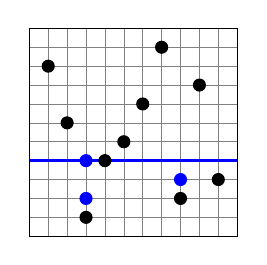
\begin{tikzpicture}[scale=0.24]
            \draw[very thin, gray] (0,0) grid (11,11);
    
            \draw[blue, line width=1.2pt] (0,4) -- (11,4);

            \filldraw[black] (3,1) circle (9pt);
            \filldraw[black] (8,2) circle (9pt);
            \filldraw[black] (10,3) circle (9pt);
            \filldraw[black] (4,4) circle (9pt);
            \filldraw[black] (5,5) circle (9pt);
            \filldraw[black] (2,6) circle (9pt);
            \filldraw[black] (6,7) circle (9pt);
            \filldraw[black] (9,8) circle (9pt);
            \filldraw[black] (1,9) circle (9pt);
            \filldraw[black] (7,10) circle (9pt);


            
            
            \filldraw[blue] (3,2) circle (9pt);
            \filldraw[blue] (8,3) circle (9pt);
            \filldraw[blue] (3,4) circle (9pt);

            \draw[black, line width=0.5pt] (0,0) rectangle (11,11); 
        \end{tikzpicture}
        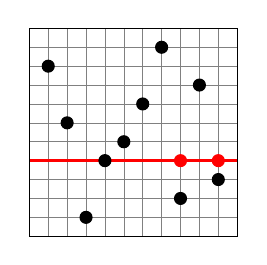
\begin{tikzpicture}[scale=0.24]
            \draw[very thin, gray] (0,0) grid (11,11);
    
            \draw[red, line width=1.2pt] (0,4) -- (11,4);

            \filldraw[black] (3,1) circle (9pt);
            \filldraw[black] (8,2) circle (9pt);
            \filldraw[black] (10,3) circle (9pt);
            \filldraw[black] (4,4) circle (9pt);
            \filldraw[black] (5,5) circle (9pt);
            \filldraw[black] (2,6) circle (9pt);
            \filldraw[black] (6,7) circle (9pt);
            \filldraw[black] (9,8) circle (9pt);
            \filldraw[black] (1,9) circle (9pt);
            \filldraw[black] (7,10) circle (9pt);

            \filldraw[red] (8,4) circle (9pt);
            \filldraw[red] (10,4) circle (9pt);

            \draw[black, line width=0.5pt] (0,0) rectangle (11,11); 
        \end{tikzpicture}
        \\
        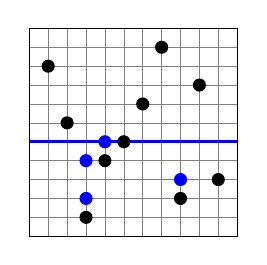
\begin{tikzpicture}[scale=0.24]
            \draw[very thin, gray] (0,0) grid (11,11);
    
            \draw[blue, line width=1.2pt] (0,5) -- (11,5);

            \filldraw[black] (3,1) circle (9pt);
            \filldraw[black] (8,2) circle (9pt);
            \filldraw[black] (10,3) circle (9pt);
            \filldraw[black] (4,4) circle (9pt);
            \filldraw[black] (5,5) circle (9pt);
            \filldraw[black] (2,6) circle (9pt);
            \filldraw[black] (6,7) circle (9pt);
            \filldraw[black] (9,8) circle (9pt);
            \filldraw[black] (1,9) circle (9pt);
            \filldraw[black] (7,10) circle (9pt);
            
            \filldraw[blue] (3,2) circle (9pt);
            \filldraw[blue] (8,3) circle (9pt);
            \filldraw[blue] (3,4) circle (9pt);
            \filldraw[blue] (4,5) circle (9pt);

            \draw[black, line width=0.5pt] (0,0) rectangle (11,11); 
        \end{tikzpicture}
        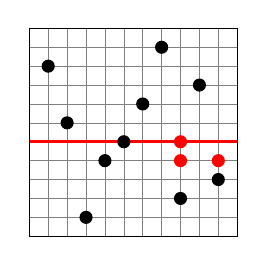
\begin{tikzpicture}[scale=0.24]
            \draw[very thin, gray] (0,0) grid (11,11);
    
            \draw[red, line width=1.2pt] (0,5) -- (11,5);

            \filldraw[black] (3,1) circle (9pt);
            \filldraw[black] (8,2) circle (9pt);
            \filldraw[black] (10,3) circle (9pt);
            \filldraw[black] (4,4) circle (9pt);
            \filldraw[black] (5,5) circle (9pt);
            \filldraw[black] (2,6) circle (9pt);
            \filldraw[black] (6,7) circle (9pt);
            \filldraw[black] (9,8) circle (9pt);
            \filldraw[black] (1,9) circle (9pt);
            \filldraw[black] (7,10) circle (9pt);
            
            \filldraw[red] (8,4) circle (9pt);
            \filldraw[red] (10,4) circle (9pt);
            \filldraw[red] (8,5) circle (9pt);

            \draw[black, line width=0.5pt] (0,0) rectangle (11,11); 
        \end{tikzpicture}
    \end{minipage}
    %\hspace{0.01\linewidth}
    \hfill
    \begin{minipage}[b]{0.48\linewidth}
        \centering
        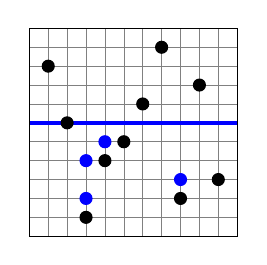
\begin{tikzpicture}[scale=0.24]
            \draw[very thin, gray] (0,0) grid (11,11);
    
            \draw[blue, line width=1.2pt] (0,6) -- (11,6);

            \filldraw[black] (3,1) circle (9pt);
            \filldraw[black] (8,2) circle (9pt);
            \filldraw[black] (10,3) circle (9pt);
            \filldraw[black] (4,4) circle (9pt);
            \filldraw[black] (5,5) circle (9pt);
            \filldraw[black] (2,6) circle (9pt);
            \filldraw[black] (6,7) circle (9pt);
            \filldraw[black] (9,8) circle (9pt);
            \filldraw[black] (1,9) circle (9pt);
            \filldraw[black] (7,10) circle (9pt);
  
            \filldraw[blue] (3,2) circle (9pt);
            \filldraw[blue] (8,3) circle (9pt);
            \filldraw[blue] (3,4) circle (9pt);
            \filldraw[blue] (4,5) circle (9pt);

            \draw[black, line width=0.5pt] (0,0) rectangle (11,11); 
        \end{tikzpicture}
        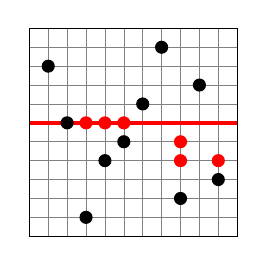
\begin{tikzpicture}[scale=0.24]
            \draw[very thin, gray] (0,0) grid (11,11);
    
            \draw[red, line width=1.2pt] (0,6) -- (11,6);

            \filldraw[black] (3,1) circle (9pt);
            \filldraw[black] (8,2) circle (9pt);
            \filldraw[black] (10,3) circle (9pt);
            \filldraw[black] (4,4) circle (9pt);
            \filldraw[black] (5,5) circle (9pt);
            \filldraw[black] (2,6) circle (9pt);
            \filldraw[black] (6,7) circle (9pt);
            \filldraw[black] (9,8) circle (9pt);
            \filldraw[black] (1,9) circle (9pt);
            \filldraw[black] (7,10) circle (9pt);
            
            \filldraw[red] (8,4) circle (9pt);
            \filldraw[red] (10,4) circle (9pt);
            \filldraw[red] (8,5) circle (9pt);
            \filldraw[red] (3,6) circle (9pt);
            \filldraw[red] (4,6) circle (9pt);
            \filldraw[red] (5,6) circle (9pt);

            \draw[black, line width=0.5pt] (0,0) rectangle (11,11); 
        \end{tikzpicture}
        \\
        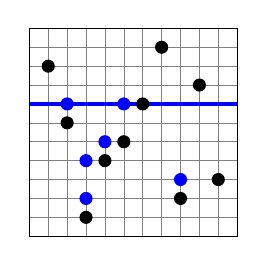
\begin{tikzpicture}[scale=0.24]
            \draw[very thin, gray] (0,0) grid (11,11);
    
            \draw[blue, line width=1.2pt] (0,7) -- (11,7);

            \filldraw[black] (3,1) circle (9pt);
            \filldraw[black] (8,2) circle (9pt);
            \filldraw[black] (10,3) circle (9pt);
            \filldraw[black] (4,4) circle (9pt);
            \filldraw[black] (5,5) circle (9pt);
            \filldraw[black] (2,6) circle (9pt);
            \filldraw[black] (6,7) circle (9pt);
            \filldraw[black] (9,8) circle (9pt);
            \filldraw[black] (1,9) circle (9pt);
            \filldraw[black] (7,10) circle (9pt);
            
            \filldraw[blue] (3,2) circle (9pt);
            \filldraw[blue] (8,3) circle (9pt);
            \filldraw[blue] (3,4) circle (9pt);
            \filldraw[blue] (4,5) circle (9pt);
            \filldraw[blue] (2,7) circle (9pt);
            \filldraw[blue] (5,7) circle (9pt);

            \draw[black, line width=0.5pt] (0,0) rectangle (11,11); 
        \end{tikzpicture}
        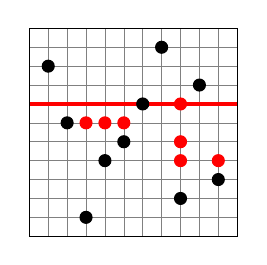
\begin{tikzpicture}[scale=0.24]
            \draw[very thin, gray] (0,0) grid (11,11);
    
            \draw[red, line width=1.2pt] (0,7) -- (11,7);

            \filldraw[black] (3,1) circle (9pt);
            \filldraw[black] (8,2) circle (9pt);
            \filldraw[black] (10,3) circle (9pt);
            \filldraw[black] (4,4) circle (9pt);
            \filldraw[black] (5,5) circle (9pt);
            \filldraw[black] (2,6) circle (9pt);
            \filldraw[black] (6,7) circle (9pt);
            \filldraw[black] (9,8) circle (9pt);
            \filldraw[black] (1,9) circle (9pt);
            \filldraw[black] (7,10) circle (9pt);
            
            \filldraw[red] (8,4) circle (9pt);
            \filldraw[red] (10,4) circle (9pt);
            \filldraw[red] (8,5) circle (9pt);
            \filldraw[red] (3,6) circle (9pt);
            \filldraw[red] (4,6) circle (9pt);
            \filldraw[red] (5,6) circle (9pt);
            \filldraw[red] (8,7) circle (9pt);

            \draw[black, line width=0.5pt] (0,0) rectangle (11,11); 
        \end{tikzpicture}   
        \\
        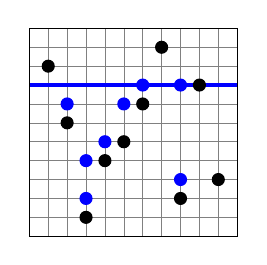
\begin{tikzpicture}[scale=0.24]
            \draw[very thin, gray] (0,0) grid (11,11);
    
            \draw[blue, line width=1.2pt] (0,8) -- (11,8);

            \filldraw[black] (3,1) circle (9pt);
            \filldraw[black] (8,2) circle (9pt);
            \filldraw[black] (10,3) circle (9pt);
            \filldraw[black] (4,4) circle (9pt);
            \filldraw[black] (5,5) circle (9pt);
            \filldraw[black] (2,6) circle (9pt);
            \filldraw[black] (6,7) circle (9pt);
            \filldraw[black] (9,8) circle (9pt);
            \filldraw[black] (1,9) circle (9pt);
            \filldraw[black] (7,10) circle (9pt);            
            
            \filldraw[blue] (3,2) circle (9pt);
            \filldraw[blue] (8,3) circle (9pt);
            \filldraw[blue] (3,4) circle (9pt);
            \filldraw[blue] (4,5) circle (9pt);
            \filldraw[blue] (2,7) circle (9pt);
            \filldraw[blue] (5,7) circle (9pt);
            \filldraw[blue] (6,8) circle (9pt);
            \filldraw[blue] (8,8) circle (9pt);

            \draw[black, line width=0.5pt] (0,0) rectangle (11,11); 
        \end{tikzpicture}
        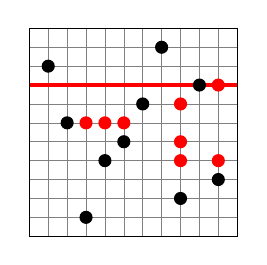
\begin{tikzpicture}[scale=0.24]
            \draw[very thin, gray] (0,0) grid (11,11);
    
            \draw[red, line width=1.2pt] (0,8) -- (11,8);

            \filldraw[black] (3,1) circle (9pt);
            \filldraw[black] (8,2) circle (9pt);
            \filldraw[black] (10,3) circle (9pt);
            \filldraw[black] (4,4) circle (9pt);
            \filldraw[black] (5,5) circle (9pt);
            \filldraw[black] (2,6) circle (9pt);
            \filldraw[black] (6,7) circle (9pt);
            \filldraw[black] (9,8) circle (9pt);
            \filldraw[black] (1,9) circle (9pt);
            \filldraw[black] (7,10) circle (9pt);

            \filldraw[red] (8,4) circle (9pt);
            \filldraw[red] (10,4) circle (9pt);
            \filldraw[red] (8,5) circle (9pt);
            \filldraw[red] (3,6) circle (9pt);
            \filldraw[red] (4,6) circle (9pt);
            \filldraw[red] (5,6) circle (9pt);
            \filldraw[red] (8,7) circle (9pt);
            \filldraw[red] (10,8) circle (9pt);

            \draw[black, line width=0.5pt] (0,0) rectangle (11,11); 
        \end{tikzpicture}
        \\
        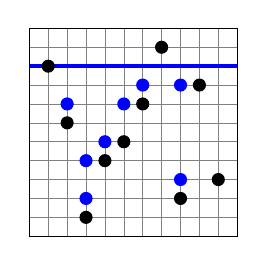
\begin{tikzpicture}[scale=0.24]
            \draw[very thin, gray] (0,0) grid (11,11);
    
            \draw[blue, line width=1.2pt] (0,9) -- (11,9);

            \filldraw[black] (3,1) circle (9pt);
            \filldraw[black] (8,2) circle (9pt);
            \filldraw[black] (10,3) circle (9pt);
            \filldraw[black] (4,4) circle (9pt);
            \filldraw[black] (5,5) circle (9pt);
            \filldraw[black] (2,6) circle (9pt);
            \filldraw[black] (6,7) circle (9pt);
            \filldraw[black] (9,8) circle (9pt);
            \filldraw[black] (1,9) circle (9pt);
            \filldraw[black] (7,10) circle (9pt);
            
            \filldraw[blue] (3,2) circle (9pt);
            \filldraw[blue] (8,3) circle (9pt);
            \filldraw[blue] (3,4) circle (9pt);
            \filldraw[blue] (4,5) circle (9pt);
            \filldraw[blue] (2,7) circle (9pt);
            \filldraw[blue] (5,7) circle (9pt);
            \filldraw[blue] (6,8) circle (9pt);
            \filldraw[blue] (8,8) circle (9pt);

            \draw[black, line width=0.5pt] (0,0) rectangle (11,11); 
        \end{tikzpicture}
        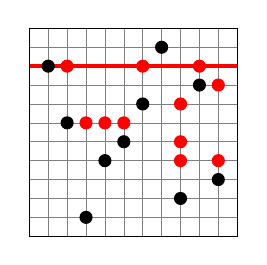
\begin{tikzpicture}[scale=0.24]
            \draw[very thin, gray] (0,0) grid (11,11);
    
            \draw[red, line width=1.2pt] (0,9) -- (11,9);

            \filldraw[black] (3,1) circle (9pt);
            \filldraw[black] (8,2) circle (9pt);
            \filldraw[black] (10,3) circle (9pt);
            \filldraw[black] (4,4) circle (9pt);
            \filldraw[black] (5,5) circle (9pt);
            \filldraw[black] (2,6) circle (9pt);
            \filldraw[black] (6,7) circle (9pt);
            \filldraw[black] (9,8) circle (9pt);
            \filldraw[black] (1,9) circle (9pt);
            \filldraw[black] (7,10) circle (9pt);

            \filldraw[red] (8,4) circle (9pt);
            \filldraw[red] (10,4) circle (9pt);
            \filldraw[red] (8,5) circle (9pt);
            \filldraw[red] (3,6) circle (9pt);
            \filldraw[red] (4,6) circle (9pt);
            \filldraw[red] (5,6) circle (9pt);
            \filldraw[red] (8,7) circle (9pt);
            \filldraw[red] (10,8) circle (9pt);
            \filldraw[red] (2,9) circle (9pt);
            \filldraw[red] (6,9) circle (9pt);
            \filldraw[red] (9,9) circle (9pt);

            \draw[black, line width=0.5pt] (0,0) rectangle (11,11); 
        \end{tikzpicture}
        \\
        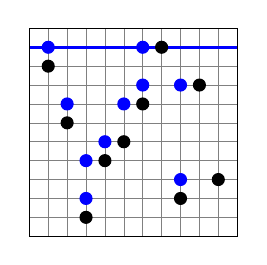
\begin{tikzpicture}[scale=0.24]
            \draw[very thin, gray] (0,0) grid (11,11);
    
            \draw[blue, line width=1.2pt] (0,10) -- (11,10);

            \filldraw[black] (3,1) circle (9pt);
            \filldraw[black] (8,2) circle (9pt);
            \filldraw[black] (10,3) circle (9pt);
            \filldraw[black] (4,4) circle (9pt);
            \filldraw[black] (5,5) circle (9pt);
            \filldraw[black] (2,6) circle (9pt);
            \filldraw[black] (6,7) circle (9pt);
            \filldraw[black] (9,8) circle (9pt);
            \filldraw[black] (1,9) circle (9pt);
            \filldraw[black] (7,10) circle (9pt);
            
            \filldraw[blue] (3,2) circle (9pt);
            \filldraw[blue] (8,3) circle (9pt);
            \filldraw[blue] (3,4) circle (9pt);
            \filldraw[blue] (4,5) circle (9pt);
            \filldraw[blue] (2,7) circle (9pt);
            \filldraw[blue] (5,7) circle (9pt);
            \filldraw[blue] (6,8) circle (9pt);
            \filldraw[blue] (8,8) circle (9pt);
            \filldraw[blue] (1,10) circle (9pt);
            \filldraw[blue] (6,10) circle (9pt);

            \draw[black, line width=0.5pt] (0,0) rectangle (11,11); 
        \end{tikzpicture}
        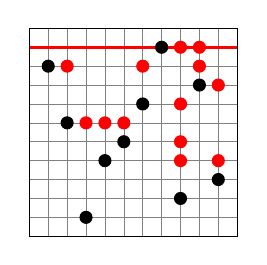
\begin{tikzpicture}[scale=0.24]
            \draw[very thin, gray] (0,0) grid (11,11);
    
            \draw[red, line width=1.2pt] (0,10) -- (11,10);

            \filldraw[black] (3,1) circle (9pt);
            \filldraw[black] (8,2) circle (9pt);
            \filldraw[black] (10,3) circle (9pt);
            \filldraw[black] (4,4) circle (9pt);
            \filldraw[black] (5,5) circle (9pt);
            \filldraw[black] (2,6) circle (9pt);
            \filldraw[black] (6,7) circle (9pt);
            \filldraw[black] (9,8) circle (9pt);
            \filldraw[black] (1,9) circle (9pt);
            \filldraw[black] (7,10) circle (9pt);
            
            \filldraw[red] (8,4) circle (9pt);
            \filldraw[red] (10,4) circle (9pt);
            \filldraw[red] (8,5) circle (9pt);
            \filldraw[red] (3,6) circle (9pt);
            \filldraw[red] (4,6) circle (9pt);
            \filldraw[red] (5,6) circle (9pt);
            \filldraw[red] (8,7) circle (9pt);
            \filldraw[red] (10,8) circle (9pt);
            \filldraw[red] (2,9) circle (9pt);
            \filldraw[red] (6,9) circle (9pt);
            \filldraw[red] (9,9) circle (9pt);
            \filldraw[red] (8,10) circle (9pt);
            \filldraw[red] (9,10) circle (9pt);

            \draw[black, line width=0.5pt] (0,0) rectangle (11,11); 
        \end{tikzpicture}
    \end{minipage}
    \caption{Em preto, o conjunto $P_X$ da sequência $X = (3,8,10,4,5,2,6,9,1,7)$ de acessos. Em azul, o conjunto obtido pelo \protect\rectpos-futurista para $P_X$ e em vermelho, o do \protect\rectneg-futurista.}
\label{fig:greedy_sign}
\end{figure}

Esse algoritmos terão um papel essencial para a última seção desse capítulo, onde buscamos delimitações inferiores de custo para sequências de acesso.

\section{Independência de retângulos}
Um conjunto $I$ de retângulos é \textit{independente} se todos os retângulos de~$I$ são arboreamente insatisfeitos e não há nenhum vértice de algum dos retângulos de $I$ estritamente no interior de outro retângulo de $I$. Veja a Figura~\ref{fig:retangulos_independentes}.

\begin{figure}[H]
    \hspace{0.05cm}
    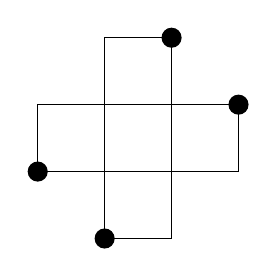
\begin{tikzpicture}[scale=0.85]
        \draw (1,1) rectangle (4,2); % Quadrado
        \draw (2,0) rectangle (3,3); % Quadrado
        \fill (2,0) circle (0.15);
        \fill (1,1) circle (0.15);
        \fill (3,3) circle (0.15);
        \fill (4,2) circle (0.15);
    \end{tikzpicture}
    \hspace{0.2cm}
    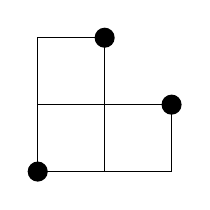
\begin{tikzpicture}[scale=0.85]
        \draw (0,0) rectangle (1,2); % Quadrado
        \draw (0,0) rectangle (2,1); % Quadrado
        \fill (0,0) circle (0.15);
        \fill (1,2) circle (0.15);
        \fill (2,1) circle (0.15);
    \end{tikzpicture}
    \hspace{0.2cm}
    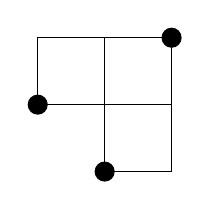
\begin{tikzpicture}[scale=0.85]
        \draw (0,1) rectangle (2,2); % Quadrado
        \draw (1,0) rectangle (2,2); % Quadrado
        \fill (0,1) circle (0.15);
        \fill (1,0) circle (0.15);
        \fill (2,2) circle (0.15);
    \end{tikzpicture}
    \hspace{0.5cm}
    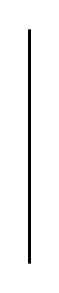
\begin{tikzpicture}[scale=0.85]
        \draw[very thick] (0,-0.5) rectangle (0,3);
    \end{tikzpicture}
    \hspace{0.5cm}
    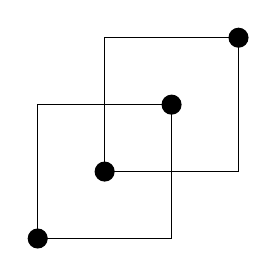
\begin{tikzpicture}[scale=0.85]
        \draw (0,0) rectangle (2,2); % Quadrado
        \draw (1,1) rectangle (3,3); % Quadrado
        \fill (0,0) circle (0.15);
        \fill (1,1) circle (0.15);
        \fill (2,2) circle (0.15);
        \fill (3,3) circle (0.15);
    \end{tikzpicture}
    \hspace{0.2cm}
    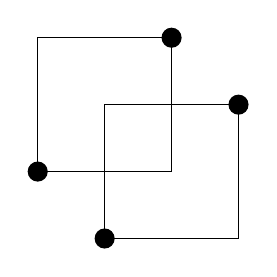
\begin{tikzpicture}[scale=0.85]
        \draw (0,1) rectangle (2,3); % Quadrado
        \draw (1,0) rectangle (3,2); % Quadrado
        \fill (0,1) circle (0.15);
        \fill (1,0) circle (0.15);
        \fill (3,2) circle (0.15);
        \fill (2,3) circle (0.15);
    \end{tikzpicture}
    \caption{Todas as combinações de dois \protect\rectpos-retângulos que compartilham área no interior. À esquerda, pares de retângulos independentes e à direita, pares retângulos dependentes.}
\label{fig:retangulos_independentes}
\end{figure}

\begin{lemma} \label{lema_6.1}
    Para toda sequência $X$ de acessos, existe um conjunto independente IRB$_{\rectpos}$$(P_X)$ de $\rectpos$-retângulos tal que $|$IRB$_{\rectpos}(P_X)| = |$Fut$_{\rectpos}(P_X)|$.
\end{lemma}

%CHEIO DE PROBLEMAS!!!
\begin{proof}
    Para todo ponto $q$ em Fut$_{\rectpos}(P_X)$, seja $R(q)$ o $\rectpos$-retângulo que o ponto $q$ satisfaz arboreamente. Sejam $r$ e $s$ os vértices desse retângulo, sendo $r$ o ponto de $P_X$ abaixo de $q$ e $s$ o ponto de $P_X$ a direita de $q$. Por construção $R(q)$ só é igual a $R(t)$ se e somente se $q = t$. Seja \( \text{IRB}_{\rectpos}(P_X) = \{ R(q) \mid q \in \text{Fut}_{\rectpos}(P_X) \} \). Obviamente $|\text{IRB}_{\rectpos}(P_X)| = |\text{Fut}_{\rectpos}(P_X)|$ e por construção nenhum ponto de Fut$_{\rectpos}(P_X) \cup P_X$ está estritamente dentro de algum retângulo de IRB$_{\rectpos}$ e o vértice superior esquerdo de todos os retângulos de $\text{IRB}_{\rectpos}(P_X)$ estão em $\text{Fut}_{\rectpos}(P_X) \cup P_X$.
\end{proof}

Para visualizar a ideia da prova acima, veja a Figura~\ref{fig:IRB_igual_add}. Note que analogamente à prova, o conjunto de $\rectpos$-retângulos independentes mostrado possui o vértice superior esquerdo localizado em algum ponto adicionado pelo algoritmo guloso futurista-$\rectpos$. 

\begin{figure}
    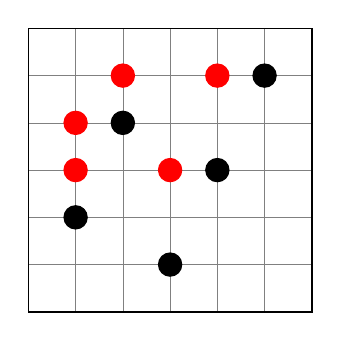
\begin{tikzpicture}[scale=0.6]
        \draw[very thin, gray] (0,0) grid (6,6);

        \filldraw[black] (3,1) circle (7pt);
        \filldraw[black] (1,2) circle (7pt);
        \filldraw[black] (4,3) circle (7pt);
        \filldraw[black] (2,4) circle (7pt);
        \filldraw[black] (5,5) circle (7pt);
        \filldraw[red] (3,3) circle (7pt);
        \filldraw[red] (1,3) circle (7pt);
        \filldraw[red] (1,4) circle (7pt);
        \filldraw[red] (2,5) circle (7pt);
        \filldraw[red] (4,5) circle (7pt);
        
        \draw[black, line width=0.5pt] (0,0) rectangle (6,6);
    \end{tikzpicture}
    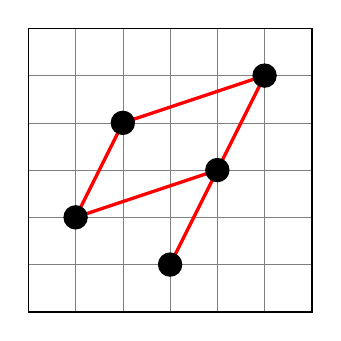
\begin{tikzpicture}[scale=0.6]
        \draw[very thin, gray] (0,0) grid (6,6);

        %\draw[red, very thick] (2,4) rectangle (5,5);
        %\draw[red, very thick] (1,2) rectangle (4,3);
        %\draw[blue, very thick] (3,1) rectangle (4,3);
        %\draw[blue, very thick] (1,2) rectangle (2,4);
        %\draw[blue, very thick] (4,3) rectangle (5,5);
        \draw[red, line width=1.2pt] (2,4) -- (5,5);
        \draw[red, line width=1.2pt] (1,2) -- (4,3);
        \draw[red, line width=1.2pt] (3,1) -- (4,3);
        \draw[red, line width=1.2pt] (1,2) -- (2,4);
        \draw[red, line width=1.2pt] (4,3) -- (5,5);

        \filldraw[black] (3,1) circle (7pt);
        \filldraw[black] (1,2) circle (7pt);
        \filldraw[black] (4,3) circle (7pt);
        \filldraw[black] (2,4) circle (7pt);
        \filldraw[black] (5,5) circle (7pt);

        \draw[black, line width=0.5pt] (0,0) rectangle (6,6);
    \end{tikzpicture}
    \caption{Em preto, os pontos de $P_X$ para a sequência de acessos $X = (3,1,4,2,5)$. À esquerda, a execução do guloso futurista-$\protect\rectpos$. À direita, está destacado um conjunto independente de $\protect\rectpos$-retângulos.}
\label{fig:IRB_igual_add}
\end{figure}

\begin{lemma} \label{lema_6.2}
    Considere um conjunto $\rectpos$-satisfeito $Y$ de pontos com x-coordenadas inteiras, dois pontos $a$ e $b$ não ortogonalmente colineares tais que $a,b \in Y$, e uma linha vertical $\ell$ com x-coordenada não inteira estritamente entre $a.x$ e $b.x$. Então, é possível encontrarmos dois pontos $p,q \in Y$ tais que $p.y = q.y$, $p$ está à esquerda de $\ell$ e $q$ está à direita de $\ell$ e não há nenhum ponto de $Y$ no segmento de reta horizontal que conecta $p$ e $q$. 
\end{lemma}

\begin{proof}
    Assuma sem perda de generalidade que $a.x < b.x$.
    Seja $p$ o ponto de $Y$ mais à direita e mais acima do $\{a,b\}$-retângulo que está à esquerda de $\ell$ e seja $q$ o ponto de $Y$ mais abaixo e mais a esquerda que esteja na mesma altura ou acima de $q$ do $\{a,b\}$-retângulo e esteja à direita de $\ell$. Esses pontos existem pois $a$ e $b$ satisfazem as restrições de $p$ e $q$ respectivamente. Por construção, $p$ está à esquerda de $\ell$ e $q$ à direita. Nota-se que $p.y = q.y$ obrigatoriamente, pois caso contrário o $\{p,q\}$-retângulo estaria insatisfeito, ou seja, existiria um $\rectpos$-retângulo insatisfeito dentro de um conjunto $Y$ de pontos $\rectpos$-satisfeito, o que é uma contradição. Veja a Figura~\ref{fig:contraexemplo_contradicao} para uma ilustração dessa contradição.
\end{proof}

\begin{figure}
    \begin{tikzpicture}[scale=1]
        \fill[pattern=north east lines, pattern color=gray](2,0) -- (3,0) -- (3,1) -- (4,1) -- (4,2) -- (3,2) -- (3,3) -- (1.8,3) -- (1.8,1) -- (2,1) -- cycle;
        \draw[very thick] (0,0) rectangle (6,3);
        \fill (0,0) circle (4pt) node[below left] {$a$};
        \fill (6,3) circle (4pt) node[above right] {$b$};
        \fill (2,1) circle (4pt) node[below left] {$p$};
        \fill (4,2) circle (4pt) node[above right] {$q$};
        \fill (3,2.5) circle (0.0001pt) node[right, red] {$\ell$};
        \draw[very thick, red] (3,0) -- (3,3);
    \end{tikzpicture}
    \caption{Um $\{a,b\}$-retângulo de um conjunto $\protect\rectpos$-satisfeito $Y$ de pontos. O ponto $p$ é o mais à direita e mais acima de $Y$ à esquerda da reta $\ell$ e o ponto $q$ é o mais à esquerda e mais abaixo que está à direita de $\ell$ e acima de $p$. A área destacada não pode conter pontos de $Y$ por conta da escolha de $p$ e $q$.}
\label{fig:contraexemplo_contradicao}
\end{figure}
\begin{lemma} \label{lema_6.3}
    Para um conjunto independente $I$ de retângulos de um conjunto $P$ de pontos tal que todo ponto tem x-coordenada distinta e inteira, existe um $\{a,b\}$-retângulo com $(a,b) \in I$, e uma reta vertical $\ell$ que cruza o eixo x num valor não inteiro estritamente entre $a.x$ e $b.x$ tal que dentro deste $\{a,b\}$-retângulo, $\ell$ não intersecta nenhum outro retângulo de $I$.
\end{lemma}

\begin{proof}
    Sejam $a$ e $b$ os dois vértice do retângulo com máxima largura em $I$, ou seja, o retângulo com maior comprimento horizontal. Assuma por simetria que $a < b$. Como $I$ é um conjunto independente de retângulos, então nenhum retângulo de $I$ possui estritamente em seu interior algum vértice de outro retângulo de $I$. 
    
    Assim, existem três tipos possíveis de retângulos de $I$ que compartilham alguma parte da área interna com o $\{a,b\}$-retângulo: o tipo-1 são os retângulos que possuem $a$ como um de seus vértices, o tipo-2 são os retângulos que possuem $b$ como um de seus vértices e o tipo-3 são os retângulos que não possuem nem $a$ nem $b$ como um de seus vértices. Note que os retângulos do tipo-3 não podem ser mais largos que o $\{a,b\}$-retângulo, pois o $\{a,b\}$-retângulo é o retângulo com máxima largura em $I$. Veja a Figura~\ref{fig:retangulo_wider} para a visualização desses três tipos.

\begin{figure}
    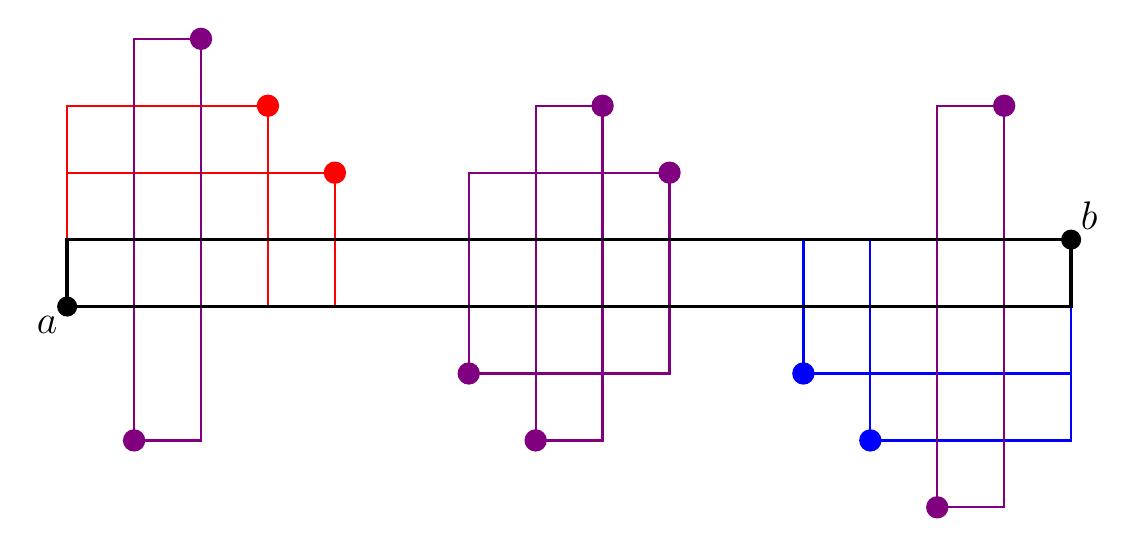
\begin{tikzpicture}[scale=0.85]
        \draw[draw=red, thick] (0,1) rectangle (4,3);
        \draw[draw=red, thick] (0,1) rectangle (3,4);
        \draw[draw=violet, thick] (1,-1) rectangle (2,5);
        
        \fill (0,1) circle (0.15);
        \node[below left] at (0,1) {\Large$a$};
        \fill (15,2) circle (0.15);
        \node[above right] at (15,2) {\Large$b$};
        \fill[draw=red, fill=red, thick] (4,3) circle (0.15);
        \fill[draw=red, fill=red, thick] (3,4) circle (0.15);
        \fill[draw=violet, fill=violet, thick] (1,-1) circle (0.15);
        \fill[draw=violet, fill=violet, thick] (2,5) circle (0.15);
        
        
        \draw[draw=violet, thick] (6,0) rectangle (9,3);
        \draw[draw=violet, thick] (7,-1) rectangle (8,4);
        \fill[draw=violet, fill=violet, thick] (6,0) circle (0.15);
        \fill[draw=violet, fill=violet, thick] (9,3) circle (0.15);
        \fill[draw=violet, fill=violet, thick] (7,-1) circle (0.15);
        \fill[draw=violet, fill=violet, thick] (8,4) circle (0.15);
        
        
        \draw[draw=blue, thick] (15,2) rectangle (11,0);
        \draw[draw=blue, thick] (15,2) rectangle (12,-1);
        \draw[draw=violet, thick] (14,-2) rectangle (13,4);
        \fill[draw=blue, fill=blue, thick] (12,-1) circle (0.15);
        \fill[draw=blue, fill=blue, thick] (11,0) circle (0.15);
        
        \fill[draw=violet, fill=violet, thick] (13,-2) circle (0.15);
        \fill[draw=violet, fill=violet, thick] (14,4) circle (0.15);
        \draw[very thick] (0,1) rectangle (15,2);
    \end{tikzpicture}
    \caption{Em preto, o $\{a,b\}$-retângulo sendo analisado. Em vermelho, os retângulos independentes que compartilham o vértice $a$. Em azul, os retângulos independentes que compartilham o vértice $b$. Em roxo, os retângulos independentes que não compartilham vértice em comum com o $\{a,b\}$-retângulo.}
\label{fig:retangulo_wider}
\end{figure}

    Perceba que só é possível a criação de 3 blocos de retângulos. À esquerda, pode ser criado um bloco de retângulos do tipo-1 e do tipo-3. Ao meio, pode ser criado um bloco de retângulos do tipo-3. À direita, pode ser criado um bloco de retângulos do tipo-2 e do tipo-3. O bloco de retângulos à esquerda e o bloco de retângulos ao meio não podem ter áreas compartilhadas, pois o conjunto $I$ é independente e o conjunto $P$ tem x-coordenada distinta. O mesmo argumento vale para mostrar que o bloco de retângulos ao meio não pode ter área compartilhada com o bloco de retângulos à direita.

    Como os pontos de $P$ possuem x-coordenada inteira, então é possível definir uma reta $\ell$ vertical que cruza o eixo x num valor não inteiro estritamente entre a x-coordenada do ponto mais a direita de $P$ pertencente a um dos retângulos do primeiro bloco e a x-coordenada do ponto mais a esquerda de $P$ pertencente a um dos retângulos do segundo bloco. O mesmo poderia ser feito para o segundo e terceiro bloco. A reta $\ell$, dentro do $\{a,b\}$-retângulo, não intersecta nenhum retângulo além do $\{a,b\}$-retângulo.
\end{proof}


\begin{lemma} \label{lema_6.4}
    Dado um conjunto independente $I$ de $\rectpos$-retângulos de um conjunto $P_X$ de pontos, qualquer superconjunto $Y$ de $P_X$ que seja $\rectpos$-satisfeito tem pelo menos cardinalidade $|I| + |P_X|$. 
\end{lemma}

\begin{proof}
    Utilizando o conjunto $I$, é possível aplicar o Lema~\ref{lema_6.3} para encontrar um $\{a,b\}$-retângulo em $I$ e uma reta vertical $\ell$, onde $\ell$ não intercepta nenhum outro retângulo dentro da área do $\{a,b\}$-retângulo. Utilizando esse $\{a,b\}$-retângulo e essa reta $\ell$, podemos aplicar o Lema~\ref{lema_6.2} para encontrar dois pontos $p,q$, com $p,q \in P$, tais que $p$ está à esquerda de $\ell$ e $q$ à direita. Assim, marcamos o par de pontos $(p,q)$, removemos o $\{a,b\}$-retângulo de $I$ e repetimos o processo até não sobrar nenhum retângulo em $I$.

    Quando removemos um $\{a,b\}$-retângulo de $I$, por conta da propriedade de toda reta vertical $\ell$ não interceptar nenhum outro retângulo dentro da área do $\{a,b\}$-retângulo analisado, então nota-se que nenhum outro retângulo de $I$ possui em seu interior simultaneamente tanto $p$ quanto $q$. Assim, nota-se que cada par de pontos só será marcado uma única vez.

    Como $P_X$ possui apenas um ponto por coordenada $y$, então para cada par de pontos marcado, no máximo um ponto pertence a $P_X$, então pelo menos um deles pertence apenas ao superconjunto $Y$. Logo, o número de pontos de $Y \setminus X$ é pelo menos o número de retângulos em $I$. 
\end{proof}

\begin{lemma}\label{lema_minASS_para_Fut}
    Para qualquer conjunto $P_X$ de pontos, minASS$_{\rectpos}(P_X) = |$Fut$_{\rectpos}(P_X)| + |P_X|$.
\end{lemma}

\begin{proof}
    Após a execução do algoritmo $\rectpos$-futurista para um conjunto de pontos $P_X$ representando a sequência de acessos $X$, o conjunto de pontos $P$ resultante desse algoritmo possui tamanho $|$Fut$_{\rectpos}(P_X)| + |P_X|$. Pelo Lema~\ref{lema_6.1}, existe um conjunto independente IRB$_{\rectpos}$$(P_X)$ de $\rectpos$-retângulos tal que $|$IRB$_{\rectpos}(P_X)| = |$Fut$_{\rectpos}(P_X)|$. Pelo Lema~\ref{lema_6.4}, como existe esse tal conjunto IRB$_{\rectpos}$$(P_X)$, então qualquer superconjunto $Y$ de $P_X$ que seja $\rectpos$-satisfeito possui cardinalidade maior ou igual a $|$IRB$_{\rectpos}$$(P_X)| + |P_X|$. Como o conjunto de pontos $P$ é $\rectpos$-satisfeito e possui tamanho $|$Fut$_{\rectpos}(P_X)| + |P_X| = |$IRB$_{\rectpos}$$(P_X)| + |P_X|$, então esse é o superconjunto $\rectpos$-satisfeito minimal de $P_X$ e minASS$_{\rectpos}(P_X) = |$Fut$_{\rectpos}(P_X)| + |P_X|$.
\end{proof}

\begin{theorem}\label{teorema_retangulos_independentes}
    Se um conjunto $P_X$ de pontos contém um conjunto independente $I$ de retângulos, então minASS$_{\recttotal}(P_X) \geq |I|/2 + |P_X|$.
\end{theorem}

\begin{proof}
    Seja $Z$ qualquer conjunto $\recttotal$-satisfeito em relação ao $P_X$, onde $Z_{\rectpos} \cup P_X$ é $\rectpos$-satisfeito e  $Z_{\rectneg} \cup P_X$ é $\rectneg$-satisfeito. Seja $I_{\rectpos}$ o conjunto independente de $\rectpos$-retângulos de $I$ e analogamente $I_{\rectneg}$ o conjunto independente de $\rectneg$-retângulos de $I$. De acordo com o Lema~\ref{lema_6.4}, $|Z_{\rectpos} \cup P_X| \geq |I_{\rectpos}| + |P_X|$ e também $|Z_{\rectneg} \cup P_X| \geq |I_{\rectneg}| + |P_X|$. Suponha por simetria que $|I_{\rectpos}| \geq |I_{\rectneg}|$, então $|I_{\rectpos}| \geq |I|/2$. Logo, $|Z| \geq |Z_{\rectpos} \cup P_X| \geq |I_{\rectpos}| + |P_X| \geq |I|/2 + |P_X|$. Como todos os conjuntos $\recttotal$-satisfeito em relação ao $P_X$ possuem essa propriedade, então o conjunto de tamanho minASS$_{\recttotal}(P_X)$ também deve ter.
\end{proof}

\section{Delimitação dos retângulos independentes}

De acordo com o Teorema~\ref{teorema_retangulos_independentes}, conjuntos independentes de retângulos estão atrelados intimamente com delimitações inferiores de custo. Assim, se conseguirmos encontrar o maior conjunto independente de retângulos, então encontraremos o melhor delimitante de custo, ou seja, o delimitante que mais se aproxima de OPT$(P_X)$.

Denotemos por maxIRB$(P_X)$ como o maior conjunto independente de retângulos para o conjunto de pontos $P_X$ que representa uma sequência $X$ de buscas. Não se sabe se há uma maneira de encontrar o valor de $|$maxIRB$(P_X)|$ em tempo polinomial, muito menos se há uma maneira de encontrar o próprio conjunto independente de retângulos.
%Uma maneira conhecida de encontrar conjuntos independentes de retângulos são as delimitações propostas por Wilber \cite{lowerbound_wilber}. Esse tema será explorado com profundidade no próximo capítulo, por ora basta saber que Alt$(P_X)$ e Funil$(P_X)$ são maneiras de encontrar conjuntos independentes de retângulos em tempo polinomial.
\begin{align*}
    \frac{1}{2}maxIRB + |P_X| &\leq minASS_{\recttotal}(P_X) \quad & \text{pelo Teorema~\ref{teorema_retangulos_independentes}},\\
    &\leq minASS_{\rectpos}(P_X) + minASS_{\rectneg}(P_X) \quad & \text{pela Equação~\ref{eq:minASStotal_menorouigual_soma_de_minASSs}},\\
    &= |Fut_{\rectpos}(P_X)| + |Fut_{\rectneg}(P_X)| + 2|P_X| \quad & \text{pelo Lema~\ref{lema_minASS_para_Fut}},\\
    &= |\text{IRB}_{\rectpos}(P_X)| + |\text{IRB}_{\rectneg}(P_X)| + 2|P_X| \quad & \text{pelo Lema~\ref{lema_6.1}},\\
    &\leq 2maxIRB + 2|P_X|,\\
    &< 2maxIRB + 4|P_X|,\\
    &\leq 4minASS_{\recttotal}(P_X) \quad & \text{pelo Teorema~\ref{teorema_retangulos_independentes}},\\
    &\leq 4minASS(P_X) \quad & \text{pela Equação~\ref{eq:minASS_orientado_menor_ou_igual_minASS}}.
\end{align*}

Uma maneira de encontrar um conjunto independente de retângulos é utilizando os algoritmos gulosos futuristas orientados. Isso será feito da seguinte maneira, rode os algoritmos $\rectpos$-futurista e $\rectneg$-futurista e escolha o que colocar mais pontos. Sabemos que todos os pontos adicionados por algum dos algoritmos gulosos futuristas orientados foram para satisfazer um retângulo insatisfeito que se traduz em um retângulo independente na entrada. Seguindo os mesmos passos da expressão acima, temos
\begin{align*}
    max\{|Fut_{\rectpos}(P_X)| + |Fut_{\rectneg}(P_X)|\} + |P_X| &\geq \frac{1}{2}(|Fut_{\rectpos}(P_X)| + |Fut_{\rectneg}(P_X)|) + |P_X|,\\
    &\geq \frac{1}{4}maxIRB + \frac{1}{2}|P_X|.
\end{align*}

Dessa maneira, o tamanho do conjunto independente de retângulos encontrado pelo melhor algoritmo guloso futurista orientado para um determinado conjunto de pontos $P_X$ está em um fator constante do tamanho maior conjunto independente de retângulos.

No próximo capítulo, veremos as delimitações inferiores de Wilber. Estas delimitações são algoritmos para delimitar custos em sequências de entradas e que conseguem encontrar conjuntos de retângulos independentes de outras maneiras. 